\section{Experimental Evaluation - Problem 2}
\label{sec:expProblem2}

\begin{figure*}[t]
    \centering
    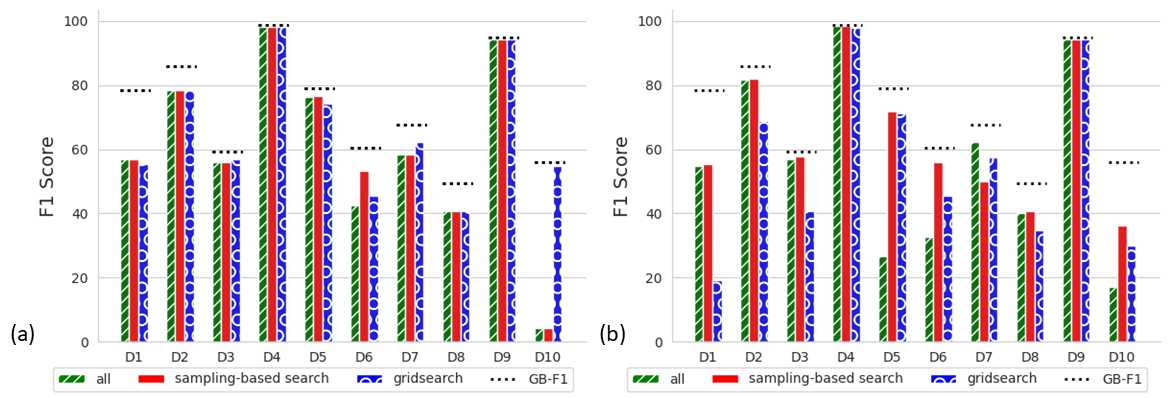
\includegraphics[width=0.9\textwidth]{Nikoletos-paper/figures/Figure7.png}
    % \vspace{-10pt}
    \caption{The F1-score of (a) the trained RF, and (b) the trained AutoML model per dataset and instance generator. GB-F1 stands for the globally best F1-score among the search algorithms in Tables \ref{tab:best-gridesearch-trials} and \ref{tab:global-bestf1s}, i.e., the performance of the best search pipeline.}
%    \vspace{-14pt}
    \label{fig:rfAutoML}
\end{figure*}
%\vspace{-3pt}
\subsection{Experimental Setup}\label{ssec:setup-p2}
For the implementation of Random Forest, we used scikit-learn v. 1.4.2\footnote{\underline{https://scikit-learn.org}}. 
For
%To implement the 
AutoML, we used auto-sklearn v. 1.4.2\footnote{\underline{https://automl.github.io/auto-sklearn}} with the following parameters: (i) The time limit in seconds for the search of appropriate models (parameter: time\_left\_for\_this\_task) was set to 12 hours. (ii) The time for a single call in the ML model (parameter: per\_run\_time\_limit) was set to 4 hours. (iii) The memory limit in MB for the machine learning algorithm (parameter: memory\_limit) equal to  24.5 GB.
%6144$\cdot$4 MB. 
(iv) The number of jobs to run in parallel (parameter: n\_jobs) was set to 1.
%No validation set used on this task, as auto-sklearn creates one internally.
All experiments were executed on a server running Ubuntu 22.04, equipped with Intel Xeon E5-4603 v2@2.2GHz and 16GB~RAM.

%\vspace{-3pt}

\subsection{Evaluation Results}
\label{sec:tackleProblem2}
%\vspace{-3pt}
To fine-tune the workflow in Figure~\ref{fig:eeter_pipeline} without any indication of matches, we apply the following procedure, resembling the leave-one-out cross-validation approach: for each dataset $D_x$ in Table~\ref{tab:dataset-specs}, we use as training set all instances generated by grid and/or sampling-based search for all other nine datasets (i.e., all datasets among $D_1$ and $D_{10}$, except $D_x$). Using these labelled instances, we train a regression model using one of the approaches in Section \ref{sec:learningProcess}. Then, we apply the learned regression model to all instances generated by the same approach for $D_x$, estimating the respective F1-score. The instance corresponding the maximum predicted F1 provides the configuration features for the ETEER pipeline that will be eventually applied to $D_x$ in order to compute the actual F1-score.

It is important to clarify the following points: 
(i) In order to find the optimal parameters, we train a model that \emph{predicts} F1-scores per configuration and picks the best one. 
(ii) After picking the best configuration, we evaluate it by computing the \emph{actual} F1 score.
(iii) Thus, we are not actually interested in the accuracy of our F1-score predictions; we are only interested in the actual F1-scores computed by using our suggested configurations.

%Note that we are not interested in measuring the accuracy of the learned model in predicting the actual F1-score per configuration; our goal is to ensure that the optimal parameter configuration is assigned the maximum predicted F1.

In this context, we address the following research questions:
\begin{enumerate}[leftmargin=*, label=RQ\arabic*), start=1]
    \item Do the three instance generation approaches in Section \ref{sec:instanceGeneration} affect the performance of the learned models?
    \item Which of the two learning processes in Section \ref{sec:learningProcess} exhibits the highest effectiveness and time efficiency?
    \item Do all features in Section \ref{sec:datasetProfiling} contribute to the effectiveness of the solutions to Problem 2?
    \item Do  our solutions to Problem 2  outperform the baseline methods w.r.t. effectiveness and time efficiency?
    \item Do our solutions to Problem 2 generalize to an unseen dataset of completely different characteristics and scale? 
    \item {How do our approaches perform in comparison to established tools for end-to-end ER that leverage syntactic similarities?}
\end{enumerate}
We elaborate on these research questions in the following.

%To address RQ4, we introduce an extra dataset (in addition to the 10 ones in Section~\ref{sec:experiments-p1}): D11, a large heterogeneous dataset which matches two different versions of DBpedia that chronologically differ by 3 years \cite{DBLP:journals/is/PapadakisMGSTGB20}.
%As baselines, we use three approaches:

%\begin{enumerate}[leftmargin=*]
%    \item The default pipeline in Table \ref{tab:best-gridesearch-trials}.
%    \item The best search pipeline, i.e., the one with the best performance for a specific dataset among the grid and sampling-based search algorithms in Tables \ref{tab:best-gridesearch-trials} and \ref{tab:global-bestf1s}, respectively. It represents the best possible performance for the ETEER pipeline of Figure~\ref{fig:eeter_pipeline}.
%    \item ZeroER \cite{DBLP:conf/sigmod/WuCSCT20}, an established ETEER approach that involves both Filtering and Verification, while requiring no labelled instances for the dataset at hand. Its performance is reported in Table \ref{tab:zeroer-results}. Note that it did not terminate in three datasets within 2 days.
%\end{enumerate}

%\begin{figure*}[t]
%    \centering
%    \begin{minipage}{0.44\linewidth}
%        \centering
%        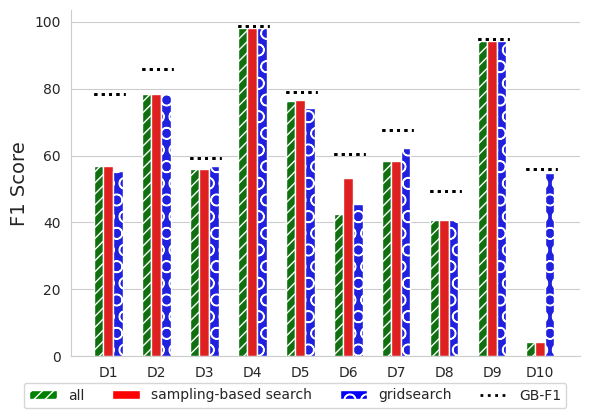
\includegraphics[width=\linewidth]{figures/predictions/sklearn_and_nn_f1.png}
        %\caption{The F1-score of the trained LR model per dataset and instance generator.}
        %\label{fig:lr-nn-f1s}
%    \end{minipage}
%    \hfill
%    \begin{minipage}{0.44\linewidth}
%        \centering
%        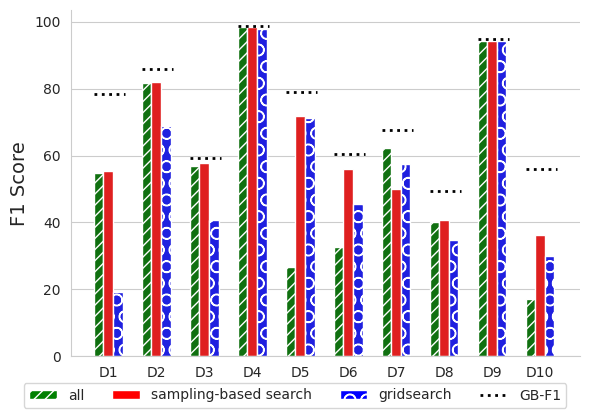
\includegraphics[width=\linewidth]{figures/predictions/autosklearn_f1.png}
        %\caption{The F1-score of the trained AutoML model per dataset and instance generator.}
%        \label{fig:autosklearnf1s}
%    \end{minipage}
%    \vspace{-10pt}
%     \caption{{\color{red}The F1-score of (a) the trained LR, and (b) the trained AutoML model per dataset and instance generator. GB-F1 stands for the globally best F1-score among the search algorithms in Tables \ref{tab:best-gridesearch-trials} and \ref{tab:global-bestf1s}, i.e., the performance of the best search pipeline.}}
%     \vspace{-10pt}
%\end{figure*}

\textbf{RQ1.} Figure \ref{fig:rfAutoML}(a) reports the F1-score of RF per dataset and instance generation approach. We observe that {the differences between the three instance generators are statistically insignificant ($p\gg0.05$ for all three pairs of generators)}. Indeed, the difference between the maximum and the minimum F1 among the three instance generators is far below 1.5\% in six of the datasets, raising to just 2.6\% and 3.6\% in $D_5$ and $D_7$, respectively. This means that there are only two datasets with significant differences between the three approaches: $D_6$, where sampling-based search takes a clear lead, and $D_{10}$, where grid search is the only approach with high performance. The extremely low performance of sampling-based search and \textit{all} on $D_{10}$ leads to \textit{grid search constituting the overall best approach for RF}, as it exhibits the highest mean F1 and the lowest variance.
%, while its distance from the globally best F1 is 10\%, on average. 
%The only exceptions appear in $D_6$ and $D_5$, where the sampling-based instances perform slightly worse and slightly better, respectively. This means that LR is able to leverage the information encapsulated in the dataset features proposed in Section \ref{sec:datasetProfiling}, regardless of the instance generator.

Much lower robustness with respect to instance generation is observed for AutoML, as shown in Figure \ref{fig:rfAutoML}(b). There is negligible deviation between the three approaches only in the two bibilographic datasets ($D_4$ and $D_9$), where the difference between the maximum and the minimum F1 is lower than 1\%. In $D_8$, this difference raises to 6\%, while in the remaining six datasets, it ranges from 12\% to 45\%. Interestingly, there is a clear winner among the three approaches: \textit{sampling-based search achieves the highest F1 in most of the datasets, while scoring the highest mean F1 and the lowest variance.} 
%On average, it also underperforms the globally best F1 by 11\%, while the other two approaches by more than 18\%.
%but $D_7$, where they rank third. In contrast, grid search instances excel in four datasets, but significantly outperform the sampling-based ones only in $D_7$.
{Indeed, the differences between sampling-based search and the other two generators are statistically significant ($p<0.05$), unlike the difference between all and grid search.}
This means that for AutoML, the 18,000 sampler instances (9 datasets $\times$ 4 search algorithms $\times$ 100 trials $\times$ 5 seeds) convey more useful information and less noise than the 359,100 grid search instances (9 datasets $\times$ 39,900 trials). 
%The combination of the two generators (``all'') typically follows the top performer or even outperforms both generators (in $D_7$).

%\begin{table*}[t]
%{\small
\begin{center}  
\caption{Performance of AutoML on Problem 2. GB stands for Gradient Boosting \cite{Friedman2001GreedyFA_GB}, KNN for K-Nearest Neighbor \cite{Fix1989DiscriminatoryA_KNN} RF for Random Forest \cite{Breiman2001RandomF_RF} and ET for Extra Trees \cite{Geurts2006ExtremelyRT_ET}. In all cases, the search/training time is 12 hours and is omitted for brevity.} 
\vspace{-10pt}
\label{tab:autosklearn-results}
%\begin{tabular}{|c|c|l|c|c|c|p{2cm}|p{1.0cm}|p{1.0cm}|c|c|c|c|}
\begin{tabular}{|c|c|l|c|c|c|c|c|c|c|}
\hline
\multirow{2}{*}{Dat.} & Inst. & \multicolumn{1}{c|}{Learned} & \multirow{2}{*}{F1} & 
%GB-F1 & F1-Ratio & 
%Optimization \& Training time (h) & 
Prediction & ETEER & \multirow{2}{*}{LM} & \multirow{2}{*}{k} & Clust & Thres \\
& gen. & \multicolumn{1}{c|}{ensemble} & & 
%GB-F1 & F1-Ratio & 
%Optimization \& Training time (h) & 
time (s) & time (s) &  &  & ering & hold \\
\hline
\hline
D1 & sampl. & 0.38ET + 0.36RF + 0.14GB + 0.1KNN + 0.02GB & 55.35 
%& 78.43 & 0.71 & 12 
& 240 & 5.84 & st5 & 1 & UMC & 0.265900 \\
D2 & sampl. & 0.82ET + 0.12GB + 0.04RF + 0.02KNN & 81.94 
%85.85 & 0.95 & 12 
& 179 & 0.18 & st5 & 1 & KC & 0.172200 \\
D3 & sampl. & 0.54ET + 0.16ET + 0.14RF + 0.12GB + 0.04KNN & 57.79 & %59.19 & 0.98 & 12 & 
218 & 2.98 & st5 & 32 & UMC & 0.05 \\
D4 & all & 0.96RF + 0.04GB & 98.45 & 
%98.60 & 1.00 & 12 & 
28 & 0.38 & st5 & 1 & CCC & 0.874200 \\
D5 & sampl. & 0.78ET + 0.1GB + 0.06RF + 0.06KNN & 71.97 & 
%78.92 & 0.91 & 12 & 
249 & 2.77 & smpnet & 1 & KC & 0.665900 \\
D6 & sampl. & 0.4ET + 0.18RF + 0.18GB + 0.12GB + 0.12KNN & 55.98 & %60.42 & 0.93 & 12 &
253 & 1.23 & sminilm & 1 & KC & 0.630700 \\
D7 & all & 0.9RF + 0.06GB + 0.04GB & 62.17 & 
%67.76 & 0.92 & 12 & 
68 & 2.05 & st5 & 1 & UMC & 0.75 \\
D8 & sampl. & 0.52ET + 0.2RF + 0.12KNN + 0.1GB + 0.06GB & 40.77 & %49.53 & 0.82 & 12 & 
230 & 20.66 & st5 & 91 & KC & 0.050100 \\
D9 & all & 0.94RF + 0.06GB & 94.39 & 
%94.92 & 0.99 & 12 & 
40 & 35.18 & st5 & 92 & KC & 0.70 \\
D10 & sampl. & 0.78ET + 0.12GB + 0.1ET & 36.31 
%& 56.12 & 0.65 & 12 
& 68 & 13.65 & smpnet & 1 & KC & 0.05 \\
\hline
\end{tabular}
\end{center}  
%}
\vspace{-10pt}
\end{table*}

%Test set & Trials training set & Regressor ensembled & F1 & GB-F1 & F1-Ratio & Optimization \& Training time (h) & Prediction time (s) & ETEER Runtime (s) & LM & k & Clustering & Threshold \\
%\midrule
%D1 & sampl. & 0.38ET + 0.36RF + 0.14GB + 0.1KNN + 0.02GB & 55.35 & 78.43 & 0.71 & 12 & 240 & 5.84 & st5 & 1 & UMC & 0.265900 \\
%D2 & sampl. & 0.82ET + 0.12GB + 0.04RF + 0.02KNN & 81.94 & 85.85 & 0.95 & 12 & 179 & 0.18 & st5 & 1 & KC & 0.172200 \\
%D3 & sampl. & 0.54ET + 0.16ET + 0.14RF + 0.12GB + 0.04KNN & 57.79 & 59.19 & 0.98 & 12 & 218 & 2.98 & st5 & 32 & UMC & 0.05 \\
%D4 & all & 0.96RF + 0.04GB & 98.45 & 98.60 & 1.00 & 12 & 28 & 0.38 & st5 & 1 & CCC & 0.874200 \\
%D5 & sampl. & 0.78ET + 0.1GB + 0.06RF + 0.06KNN & 71.97 & 78.92 & 0.91 & 12 & 249 & 2.77 & smpnet & 1 & KC & 0.665900 \\
%D6 & sampl. & 0.4ET + 0.18RF + 0.18GB + 0.12GB + 0.12KNN & 55.98 & 60.42 & 0.93 & 12 & 253 & 1.23 & sminilm & 1 & KC & 0.630700 \\
%D7 & all & 0.9RF + 0.06GB + 0.04GB & 62.17 & 67.76 & 0.92 & 12 & 68 & 2.05 & st5 & 1 & UMC & 0.75 \\
%D8 & sampl. & 0.52ET + 0.2RF + 0.12KNN + 0.1GB + 0.06GB & 40.77 & 49.53 & 0.82 & 12 & 230 & 20.66 & st5 & 91 & KC & 0.050100 \\
%D9 & all & 0.94RF + 0.06GB & 94.39 & 94.92 & 0.99 & 12 & 40 & 35.18 & st5 & 92 & KC & 0.70 \\
%D10 & sampl. & 0.78ET + 0.12GB + 0.1ET & 36.31 & 56.12 & 0.65 & 12 & 68 & 13.65 & smpnet & 1 & KC & 0.05 \\

\begin{table*}[t]
%{\small
\begin{center}  
\footnotesize  
\setlength{\tabcolsep}{2pt}
\caption{Performance of AutoML on Problem 2 when combined with sampling-based instances. GB stands for Gradient Boosting \cite{Friedman2001GreedyFA_GB}, KNN for K-Nearest Neighbor \cite{Fix1989DiscriminatoryA_KNN} RF for Random Forest \cite{Breiman2001RandomF_RF} and ET for Extra Trees \cite{Geurts2006ExtremelyRT_ET}. In all cases, the search/training time is 12 hours and is omitted for brevity.} 
% \vspace{-10pt}
{\small
\label{tab:autosklearn-results}
%\begin{tabular}{|c|c|l|c|c|c|p{2cm}|p{1.0cm}|p{1.0cm}|c|c|c|c|}
\begin{tabular}{|c|l|c|c|c|c|c|c|c|}
\hline
Dataset &  \multicolumn{1}{c|}{Learned ensemble} & F1 & 
%GB-F1 & F1-Ratio & 
%Optimization \& Training time (h) & 
Prediction time (s)& ETEER time (s)& LM & k & Clustering & Threshold \\
% & \multicolumn{1}{c|}{ensemble} & & 
%GB-F1 & F1-Ratio & 
%Optimization \& Training time (h) & 
%time (s) & time (s) &  &  & ering & hold \\
\hline
\hline
D1 & 0.38ET + 0.36RF + 0.14GB + 0.1KNN + 0.02GB & 55.35 & 240 & 5.84 & st5 & 1 & UMC & 0.2659 \\
D2 & 0.82ET + 0.12GB + 0.04RF + 0.02KNN & 81.94 & 179 & 0.18 & st5 & 1 & KC & 0.1722 \\
D3 & 0.54ET + 0.16ET + 0.14RF + 0.12GB + 0.04KNN & 57.79 & 218 & 2.98 & st5 & 32 & UMC & 0.05 \\
D4 & 0.5ET + 0.38RF + 0.08GB + 0.04KNN & 98.38 & 215 & 0.83 & st5 & 1 & KC & 0.05 \\
D5 & 0.78ET + 0.1GB + 0.06RF + 0.06KNN & 71.97 & 249 & 2.77 & smpnet & 1 & KC & 0.6659 \\
D6 & 0.4ET + 0.18RF + 0.18GB + 0.12GB + 0.12KNN & 55.98 & 253 & 1.23 & sminilm & 1 & KC & 0.6307 \\
D7 & 0.5ET + 0.24RF + 0.2GB + 0.04KNN + 0.02GB & 50.14 & 227 & 2.28 & smpnet & 1 & UMC & 0.228 \\
D8 & 0.52ET + 0.2RF + 0.12KNN + 0.1GB + 0.06GB & 40.77 & 230 & 20.66 & st5 & 91 & KC & 0.0501 \\
D9 & 0.52ET + 0.28RF + 0.14GB + 0.06KNN & 94.37 & 222 & 61.16 & st5 & 100 & KC & 0.4767 \\
D10 & 0.78ET + 0.12GB + 0.1ET & 36.31 & 68 & 13.65 & smpnet & 1 & KC & 0.05 \\
\hline
\end{tabular}
}
\end{center}  
\end{table*}
%Test set & Trials training set & Regressor ensembled & F1 & GB-F1 & F1-Ratio & Optimization \& Training time (h) & Prediction time (s) & ETEER Runtime (s) & LM & k & Clustering & Threshold \\
%\midrule
%D1 & sampl. & 0.38ET + 0.36RF + 0.14GB + 0.1KNN + 0.02GB & 55.35 & 78.43 & 0.71 & 12 & 240 & 5.84 & st5 & 1 & UMC & 0.265900 \\
%D2 & sampl. & 0.82ET + 0.12GB + 0.04RF + 0.02KNN & 81.94 & 85.85 & 0.95 & 12 & 179 & 0.18 & st5 & 1 & KC & 0.172200 \\
%D3 & sampl. & 0.54ET + 0.16ET + 0.14RF + 0.12GB + 0.04KNN & 57.79 & 59.19 & 0.98 & 12 & 218 & 2.98 & st5 & 32 & UMC & 0.05 \\
%D4 & all & 0.96RF + 0.04GB & 98.45 & 98.60 & 1.00 & 12 & 28 & 0.38 & st5 & 1 & CCC & 0.874200 \\
%D5 & sampl. & 0.78ET + 0.1GB + 0.06RF + 0.06KNN & 71.97 & 78.92 & 0.91 & 12 & 249 & 2.77 & smpnet & 1 & KC & 0.665900 \\
%D6 & sampl. & 0.4ET + 0.18RF + 0.18GB + 0.12GB + 0.12KNN & 55.98 & 60.42 & 0.93 & 12 & 253 & 1.23 & sminilm & 1 & KC & 0.630700 \\
%D7 & all & 0.9RF + 0.06GB + 0.04GB & 62.17 & 67.76 & 0.92 & 12 & 68 & 2.05 & st5 & 1 & UMC & 0.75 \\
%D8 & sampl. & 0.52ET + 0.2RF + 0.12KNN + 0.1GB + 0.06GB & 40.77 & 49.53 & 0.82 & 12 & 230 & 20.66 & st5 & 91 & KC & 0.050100 \\
%D9 & all & 0.94RF + 0.06GB & 94.39 & 94.92 & 0.99 & 12 & 40 & 35.18 & st5 & 92 & KC & 0.70 \\
%D10 & sampl. & 0.78ET + 0.12GB + 0.1ET & 36.31 & 56.12 & 0.65 & 12 & 68 & 13.65 & smpnet & 1 & KC & 0.05 \\

%\begin{table}[t]
{\small
\begin{center}  
\setlength{\tabcolsep}{2pt}
\caption{Performance of Random Forest on Problem 2.} 
\vspace{-10pt}
\label{tab:lr-with-data-features}
\begin{tabular}{|c|c|c|c|c|c|c|c|c|c|}
\hline
\multirow{2}{*}{Dat.} & Insta. & \multirow{2}{*}{F1} & Train.  & Predic.  & ETEER  & \multirow{2}{*}{LM} & \multirow{2}{*}{k} & Clust & Thre \\
 & gen. & & time (s) & time (s) &  time (s) &  &  & ering & shold \\
\hline
\hline
D1 & all & 56.77 & 0.72 & 0.02 & 2.88 & st5 & 1 & UMC & 0.73 \\
D2 & grid. & 78.46 & 0.91 & 0.01 & 5.10 & st5 & 16 & KC & 0.10 \\
D3 & grid. & 56.86 & 0.96 & 0.01 & 0.55 & st5 & 2 & KC & 0.60 \\
D4 & grid. & 98.24 & 1.00 & 0.01 & 1.70 & st5 & 2 & KC & 0.20 \\
D5 & opt. & 76.75 & 0.97 & $\ll$0.01 & 1.91 & sminilm & 1 & UMC & 0.65 \\
D6 & opt. & 53.31 & 0.88 & 0.01 & 1.34 & sminilm & 1 & KC & 0.65 \\
D7 & grid. & 62.12 & 0.92 & 0.01 & 1.58 & sminilm & 1 & KC & 0.60 \\
D8 & all & 40.78 & 0.82 & 0.01 & 28.79 & st5 & 100 & KC & 0.22 \\
D9 & all & 94.37 & 0.99 & 0.01 & 60.20 & st5 & 100 & KC & 0.38 \\
D10 & grid. & 54.91 & 0.98 & 0.01 & 37.55 & st5 & 27 & KC & 0.50 \\
\hline
\end{tabular}
\end{center}  
}
\vspace{-10pt}
\end{table}
%\toprule
% D1 & all & RFR & 56.77 & 78.43 & 0.72 & 130.55 & 1.60 & 2.88 & st5 & 1 & UMC & 0.733563 \\
% D2 & gridsearch & RFR & 78.46 & 85.85 & 0.91 & 10.10 & 0.18 & 5.10 & st5 & 16 & KC & 0.10 \\
% D3 & gridsearch & RFR & 56.86 & 59.19 & 0.96 & 10.22 & 0.18 & 0.55 & st5 & 2 & KC & 0.60 \\
% D4 & gridsearch & RFR & 98.24 & 98.60 & 1.00 & 65.26 & 1.00 & 1.70 & st5 & 2 & KC & 0.20 \\
% D5 & optuna & RFR & 76.75 & 78.92 & 0.97 & 5.25 & 0.05 & 1.91 & sminilm & 1 & UMC & 0.651879 \\
% D6 & optuna & RFR & 53.31 & 60.42 & 0.88 & 20.30 & 0.19 & 1.34 & sminilm & 1 & KC & 0.647542 \\
% D7 & gridsearch & RFR & 62.12 & 67.76 & 0.92 & 38.81 & 0.47 & 1.58 & sminilm & 1 & KC & 0.60 \\
% D8 & all & RFR & 40.78 & 49.53 & 0.82 & 27.48 & 0.29 & 28.79 & st5 & 100 & KC & 0.219945 \\
% D9 & all & RFR & 94.37 & 94.92 & 0.99 & 67.96 & 0.80 & 60.20 & st5 & 100 & KC & 0.375625 \\
% D10 & gridsearch & RFR & 54.91 & 56.12 & 0.98 & 48.67 & 0.67 & 37.55 & st5 & 27 & KC & 0.50 \\
%Test set & Trials training set & Regressor & F1 & GB-F1 & F1-Ratio & Training time (s) & Prediction time (s) & ETEER runtime (s) & LM & k & Clustering & Threshold \\
%\midrule
%D1 & all & LR & 55.35 & 78.43 & 0.71 & 0.33 & 0.01 & 0.24 & st5 & 1 & KC & 0.05 \\
%D2 & all & LR & 81.94 & 85.85 & 0.95 & 0.24 & $\ll$0.01 & 0.20 & st5 & 1 & KC & 0.05 \\
%D3 & all & LR & 55.98 & 59.19 & 0.95 & 0.33 & $\ll$0.01 & 0.48 & st5 & 1 & KC & 0.05 \\
%D4 & all & LR & 98.38 & 98.60 & 1.00 & 0.21 & $\ll$0.01 & 0.83 & st5 & 1 & KC & 0.05 \\
%D5 & all & LR & 69.39 & 78.92 & 0.88 & 0.21 & $\ll$0.01 & 0.79 & st5 & 1 & KC & 0.05 \\
%D6 & optuna & LR & 46.65 & 60.42 & 0.77 & 0.06 & $\ll$0.01 & 10.24 & st5 & 100 & KC & 0.05 \\
%D7 & all & LR & 48.48 & 67.76 & 0.72 & 0.21 & $\ll$0.01 & 1.62 & st5 & 1 & KC & 0.05 \\
%D8 & all & LR & 38.09 & 49.53 & 0.77 & 0.21 & $\ll$0.01 & 1.63 & st5 & 1 & KC & 0.05 \\
%D9 & all & LR & 92.85 & 94.92 & 0.98 & 0.21 & $\ll$0.01 & 4.23 & st5 & 1 & KC & 0.05 \\
%D10 & gridsearch & LR & 55.40 & 56.12 & 0.99 & 0.22 & 0.01 & 12.54 & st5 & 1 & KC & 0.05 \\
%\bottomrule

\begin{table}[t]
\begin{center}  
\footnotesize 
\setlength{\tabcolsep}{4pt}
\caption{Performance of Random Forest on Problem 2 when combined with grid search instances.} 
% \vspace{-10pt}
\label{tab:lr-with-data-features}
\begin{tabular}{|c|c|c|c|c|c|c|c|c|}
\hline
\multirow{2}{*}{Dat.}  & \multirow{2}{*}{F1} & Train.  & Predic.  & ETEER  & \multirow{2}{*}{LM} & \multirow{2}{*}{k} & Clust & Thre \\
 & & time (s) & time (s) &  time (s) &  &  & ering & shold \\
\hline
\hline
D1 & 55.35 & 73.10 & 1.21 & 4.11 & st5 & 1 & KC & 0.20 \\
D2 & 78.46 & 10.10 & 0.18 & 5.10 & st5 & 16 & KC & 0.10 \\
D3 & 56.86 & 10.22 & 0.18 & 0.55 & st5 & 2 & KC & 0.60 \\
D4 & 98.24 & 65.26 & 1.00 & 1.70 & st5 & 2 & KC & 0.20 \\
D5 & 74.16 & 53.34 & 0.94 & 2.05 & sminilm & 1 & KC & 0.70 \\
D6 & 45.44 & 42.50 & 0.51 & 1.20 & sminilm & 1 & KC & 0.70 \\
D7 & 62.12 & 38.81 & 0.47 & 1.58 & sminilm & 1 & KC & 0.60 \\
D8 & 40.78 & 24.27 & 0.28 & 33.10 & st5 & 99 & KC & 0.25 \\
D9 & 94.35 & 42.14 & 0.54 & 60.76 & st5 & 74 & KC & 0.35 \\
D10 & 54.91 & 48.67 & 0.67 & 37.55 & st5 & 27 & KC & 0.50 \\
\hline
\end{tabular}
\end{center}  
\end{table}
%\toprule
% D1 & all & RFR & 56.77 & 78.43 & 0.72 & 130.55 & 1.60 & 2.88 & st5 & 1 & UMC & 0.733563 \\
% D2 & gridsearch & RFR & 78.46 & 85.85 & 0.91 & 10.10 & 0.18 & 5.10 & st5 & 16 & KC & 0.10 \\
% D3 & gridsearch & RFR & 56.86 & 59.19 & 0.96 & 10.22 & 0.18 & 0.55 & st5 & 2 & KC & 0.60 \\
% D4 & gridsearch & RFR & 98.24 & 98.60 & 1.00 & 65.26 & 1.00 & 1.70 & st5 & 2 & KC & 0.20 \\
% D5 & optuna & RFR & 76.75 & 78.92 & 0.97 & 5.25 & 0.05 & 1.91 & sminilm & 1 & UMC & 0.651879 \\
% D6 & optuna & RFR & 53.31 & 60.42 & 0.88 & 20.30 & 0.19 & 1.34 & sminilm & 1 & KC & 0.647542 \\
% D7 & gridsearch & RFR & 62.12 & 67.76 & 0.92 & 38.81 & 0.47 & 1.58 & sminilm & 1 & KC & 0.60 \\
% D8 & all & RFR & 40.78 & 49.53 & 0.82 & 27.48 & 0.29 & 28.79 & st5 & 100 & KC & 0.219945 \\
% D9 & all & RFR & 94.37 & 94.92 & 0.99 & 67.96 & 0.80 & 60.20 & st5 & 100 & KC & 0.375625 \\
% D10 & gridsearch & RFR & 54.91 & 56.12 & 0.98 & 48.67 & 0.67 & 37.55 & st5 & 27 & KC & 0.50 \\
%Test set & Trials training set & Regressor & F1 & GB-F1 & F1-Ratio & Training time (s) & Prediction time (s) & ETEER runtime (s) & LM & k & Clustering & Threshold \\
%\midrule
%D1 & all & LR & 55.35 & 78.43 & 0.71 & 0.33 & 0.01 & 0.24 & st5 & 1 & KC & 0.05 \\
%D2 & all & LR & 81.94 & 85.85 & 0.95 & 0.24 & $\ll$0.01 & 0.20 & st5 & 1 & KC & 0.05 \\
%D3 & all & LR & 55.98 & 59.19 & 0.95 & 0.33 & $\ll$0.01 & 0.48 & st5 & 1 & KC & 0.05 \\
%D4 & all & LR & 98.38 & 98.60 & 1.00 & 0.21 & $\ll$0.01 & 0.83 & st5 & 1 & KC & 0.05 \\
%D5 & all & LR & 69.39 & 78.92 & 0.88 & 0.21 & $\ll$0.01 & 0.79 & st5 & 1 & KC & 0.05 \\
%D6 & optuna & LR & 46.65 & 60.42 & 0.77 & 0.06 & $\ll$0.01 & 10.24 & st5 & 100 & KC & 0.05 \\
%D7 & all & LR & 48.48 & 67.76 & 0.72 & 0.21 & $\ll$0.01 & 1.62 & st5 & 1 & KC & 0.05 \\
%D8 & all & LR & 38.09 & 49.53 & 0.77 & 0.21 & $\ll$0.01 & 1.63 & st5 & 1 & KC & 0.05 \\
%D9 & all & LR & 92.85 & 94.92 & 0.98 & 0.21 & $\ll$0.01 & 4.23 & st5 & 1 & KC & 0.05 \\
%D10 & gridsearch & LR & 55.40 & 56.12 & 0.99 & 0.22 & 0.01 & 12.54 & st5 & 1 & KC & 0.05 \\
%\bottomrule

\textbf{RQ2.} We now compare the two learning processes in combination with their best instance generation approach. The performance of Random Forest with grid search instances along with the selected workflow configurations 
%for the workflow in Figure \ref{fig:eeter_pipeline} 
is reported in Table \ref{tab:lr-with-data-features}. The same information for AutoML in combination with sampling-based instances is reported in Table \ref{tab:autosklearn-results}. We observe significant variations between the selected configurations of the two learners for each dataset.

Regarding their effectiveness, the two learners exhibit practically identical F1 score in half the datasets. In fact, the difference in their F1 score is far less than 1\% in $D_1$, $D_3$, $D_4$, $D_8$ and $D_9$. AutoML takes the lead in $D_2$ and $D_6$, while Random Forest outperforms it in the three remaining datasets. {Overall, their difference is statistically insignificant ($p = 0.50651$).} With respect to average F1 score, Random Forest takes a significant lead (66.1 vs 64.3), while exhibiting lower variance. It should be stressed that \textit{AutoML's performance depends heavily on the available search/training time}, with higher budgets yielding even better results. Yet, the current limit of 12 hours is already too high when compared to the ETEER runtime, which does not exceed 36 seconds in any of the datasets.

Regarding time efficiency, Random Forest is clearly the top performer. Its training time is consistently lower than two seconds, unlike the 12 hours required by AutoML. Its prediction time is also extremely fast, consistently requiring less than 20 milliseconds, whereas AutoML typically takes a few minutes. This should be attributed to the simpler models learned by Random Forest, unlike the complicated, weighted ensemble learned by AutoML. 

For these reasons, Random Forest trained on grid search instances is the preferred approach to tackle Problem 2 and answer RQ3. Based on RF, the overall approach for training the regression model on an existing dataset, generating the testing instances to yield a workflow configuration and applying it to a specific dataset takes less than three minutes in all datasets of Table \ref{tab:lr-with-data-features}. 

\begin{figure}[t]
    \centering
    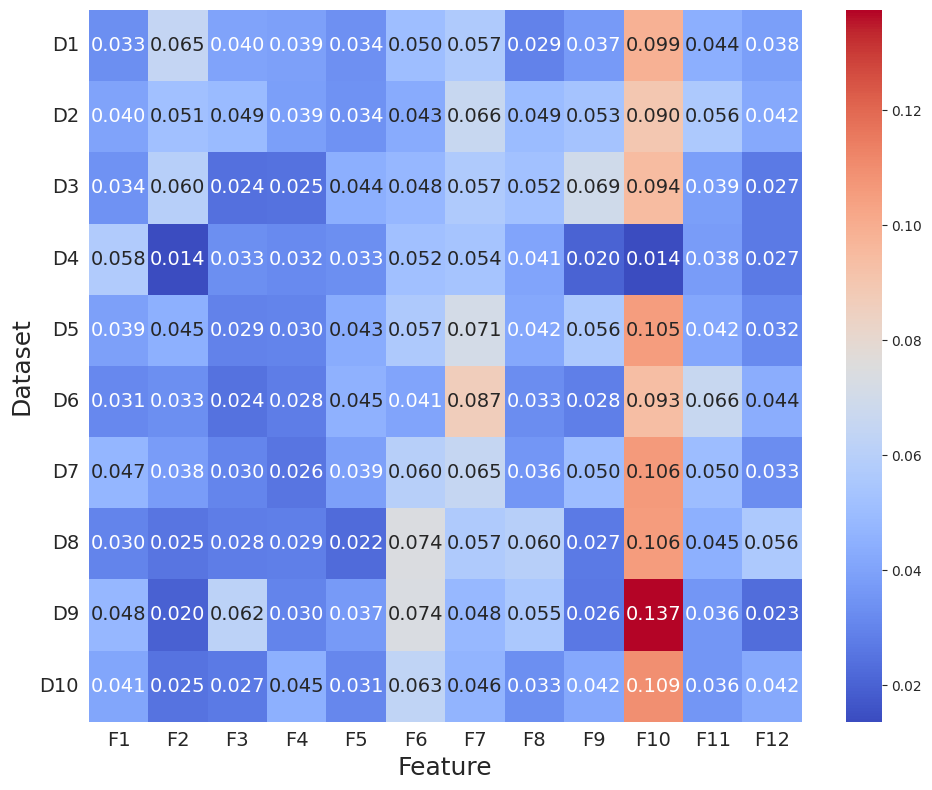
\includegraphics[width=0.85\linewidth]{Nikoletos-paper/figures/gini.png}
    % \vspace{-12pt}
    \caption{The gini importance of each feature per dataset for Random Forest with grid search instances.}
%    \vspace{-18pt}
    \label{fig:gini}
\end{figure}

\begin{table*}[t]
%\footnotesize
\centering
\setlength{\tabcolsep}{1.4pt}
\caption{Performance of ZeroER over the datasets of Table \ref{tab:dataset-specs}.}
\label{tab:zeroer-results}
\begin{tabular}{|l|c|c|c|c|c|c|c|c|c|c|}
\cline{2-11}
\multicolumn{1}{c|}{} & D1 & D2 & D3 & D4 & D5 & D6 & D7 & D8 & D9 & D10 \\
\hline
\hline
RT & 4 sec & 70 min & $\gg$48 hrs & 5.5 hrs & 34 min & $\gg$48 hrs & 67 min & $\gg$48 hrs & 24.5 hrs & 26 min \\
F1 & 0.00 & 46.46 & - & 97.00 & 92.79 & - & 88.07 & - & 64.06 & 92.62 \\
\hline
\end{tabular}
\end{table*}

\textbf{RQ3.} A major advantage of Random Forest is the interpretability of its trained decision trees, which allows for examining the specific features that are actually useful in predicting the best workflow configuration per dataset. In fact, Gini importance provides normalized estimations of the importance of each feature in $[0,1]$, with higher values indicating more important features. 

Figure \ref{fig:gini} reports this measure for all features of Section \ref{sec:datasetProfiling} across all datasets when training Random Forest with grid search instances. \textit{All features have a non-zero importance} that fluctuates between 0.137 and 0.014. On average, the most important features are F10 (0.095), F7 (0.061) and F6 (0.056), while the least important ones are F4 0.032) and F3 (0.035). Hence, \textit{despite the seemingly small variations, some features are two or even three times more important than others}. Random Forest inherently addresses these variations without requiring a specialized feature selection approach.

\begin{table*}[t]
\setlength{\tabcolsep}{3pt}
%\footnotesize
\centering
\caption{Performance over $D_{11}$ in the context of Problem 2.
%{\color{red}  ETEER Runtime (h): xana trexv ta grid,all,optuna gia na parv xronous me pre calcualated embeddings gia na mhn exei diafora me ta alla.. } 
}
% \vspace{-8pt}
\label{tab:dbpedia-results}
\begin{tabular}{|c|c|c|c|c|c|c|c|c|}
\hline
\multirow{2}{*}{LM} & \multirow{2}{*}{K} & Cluste & Thres & Training & Prediction & F1 & ETEER  & Inst. \\
 & & ring & hold& Time (h) & Time (s) & score & Runtime (h) &  gen. \\
\hline
\hline
st5 & 10 & UMC & 0.50 & - & - & 83.22 & 14.66 & - \\
\hline
\multicolumn{9}{c}{(a) Default configuration}\\
\hline
st5 & 51 & KC & 0.15 & 0.02 & 1.00 & 84.89 & 18.04 & grid \\
st5 & 1 & KC & 0.55 & 0.00 & 0.45 & 84.83 & 13.37 & sampl. \\
st5 & 100 & KC & 0.30 & 0.03 & 0.61 & 84.98 & 15.97 & all \\
\hline
\multicolumn{9}{c}{(b) Random Forest}\\
\hline
smpnet & 85 & KC & 0.55 & 12 & 17.22 & 74.26 & 16.93 & grid. \\
st5 & 1 & KC & 0.05 & 12 & 15.54 & 84.84 & 13.40 & sampl. \\
st5 & 18 & KC & 0.05 & 12 & 13.07 & 84.84 & 16.93 &  all \\
\hline
\multicolumn{9}{c}{(c) AutoML}
\end{tabular}
\vspace{-9pt}
\end{table*} 

\textbf{RQ4.} We now compare the top learned models, i.e.,  RF in combination with grid search instances and AutoML in combination with sampling-based search, with the following three baselines methods:

(i) The default pipeline in Section \ref{sec:tackleProblem1}. In most datasets, this approach underperforms both RF and AutoML to a significant extent, due to its fixed configuration. The only exception is $D_2$, where the default configuration is almost the same as the best one. AutoML performs much worse than the default configuration in $D_{10}$, too, due to the high levels of noise and the low portion of top performing configurations (see Figure \ref{fig:f1_boxplot_all}), which call for much higher search times. Overall, \textit{the adaptive workflow configurations proposed by RF and AutoML typically outperform the top-performing default one}.

(ii) The best search pipeline, i.e., GB-F1 in Figure \ref{fig:rfAutoML}, which corresponds to the best performance of the ETEER pipeline in Figure~\ref{fig:eeter_pipeline} for a specific dataset among the grid and sampling-based search algorithms in Tables \ref{tab:best-gridesearch-trials} and \ref{tab:global-bestf1s}, respectively.
%, which represents the best possible performance for the ETEER pipeline of Figure~\ref{fig:eeter_pipeline}.
%The second baseline one is the globally best F1-score among the search algorithms in Tables \ref{tab:best-gridesearch-trials} and \ref{tab:global-bestf1s} (i.e., GB-F1 in Figure \ref{fig:rfAutoML}). 
We observe that neither RF in combination with grid search instances nor AutoML in combination with sampling-based search instances outperform GB-F1 in any dataset. Yet, both RF and AutoML almost match GB-F1 in three datasets: $D_3$, $D_4$ and $D_9$. This is expected for the last two, the relatively clean bibliographic datasets, given the large portion of workflow configurations with very high performance in Figure \ref{fig:f1_boxplot_all}. For $D_{3}$, this shows the high effectiveness of both RF and AutoML. The worst performance of RF and AutoML with respect to this baseline corresponds to $D_1$ and $D_8$, where their F1-score is lower by $\sim$30\% and $\sim$20\%, respectively. These are the datasets with the lowest portion of duplicate entities, causing the selected workflow configurations to suffer from low precision. AutoML performs poorly in $D_{10}$, too, for reasons explained above.
%due to the high levels of noise and the low portion of top performing configurations (see Figure \ref{fig:f1_boxplot_all}), which call for much higher search times. 
All other datasets lie in the middle of these two extremes, with RF and AutoML underperforming GB-F1 by 10\% and 11\%, on average, respectively. 

%Random Forest, its best performance per dataset is reported in Table \ref{tab:lr-with-data-features}. It is very close to the best search pipeline in half the datasets, with LR achieving the same performance in the relatively clean bibliographic datasets, $D_4$ and $D_9$, as well as in $D_{10}$. In $D_2$ and $D_3$, its F1-score is less than 5\% lower than that of the best search pipeline. In contrast, LR underperforms almost by 30\% in $D_1$ and $D_8$, which are quite challenging, due to the very low portion of top performing configurations, as shown in Figure~\ref{fig:f1_boxplot_all}. In the remaining datasets, its F1-score is lower than the best search one by 23\% ($D_6$ and $D_8$) and 12\% ($D_5$). Overall, \textit{LR provides a performance close to the best possible one for the workflow in Figure~\ref{fig:eeter_pipeline} in most cases, while its run-time is consistently very low}, up to 21 seconds over the largest dataset, $D_{10}$. It is worth noting at this point the variety of parameter configurations proposed by LR in
%: as shown in 
%Table \ref{tab:lr-with-data-features}.
%, its overall run-time is consistently lower than the baseline methods in all datasets but $D_6$, where it uses the maximum number of candidates per query entity (100 vs 1 of the baseline methods).
%respet ETEER run-times in Table \ref{tab:best-gridesearch-trials} and most ones in Table~\ref{tab:global-bestf1s}.

(iii) ZeroER \cite{DBLP:conf/sigmod/WuCSCT20}, an established ETEER approach that involves both Filtering and Verification, while requiring no labelled instances for the dataset at hand. Its performance is reported in Table \ref{tab:zeroer-results}. Note that it did not terminate in three datasets within 2 days.
Compared to ZeroER, RF is consistently much faster: it requires far less than 3 minutes in all cases, while ZeroER requires at least 26 min in all datasets but the smallest one, where it actually finds no matches. The reason is that ZeroER cannot support missing and misplaced values, which abound in $D_1$. Apart from this dataset, RF significantly outperforms ZeroER in terms of effectiveness in three more datasets: $D_2$, $D_4$ and $D_9$. The reason is that those datasets convey long textual values, which are ideal for the pre-trained language model that lies at the core the ETEER pipeline in Figure \ref{fig:eeter_pipeline}. In contrast, $D_5$, $D_7$ and $D_{10}$ convey short textual values that usually correspond to person names. The language models struggle to find semantic similarities in these settings, unlike the string similarity measures that lie at the core of ZeroER. As a result, RF significantly underperforms ZeroER in these three datasets, but remains faster by orders of magnitude.

%Regarding AutoML, its performance is reported in Table \ref{tab:autosklearn-results}. Apart from the much higher training time (12 hours), it also raises the prediction time, due to the much more complex model that results from its learning. As a result, its performance is higher than LR in most cases, i.e., in six datasets; in $D_1$, $D_2$ and $D_4$, they yield the same F1, and only in $D_{10}$ LR performs better. Compared to the best search pipeline, the F1 score of its fine-tuned ETEER pipelines is lower by (far) less than 10\% in seven datasets. The difference is significant only in $D_1$ and $D_8$, due to the very low portion of top performing pipelines, as well as in $D_{10}$. 

Compared to ZeroER, AutoML achieves higher F1-score in the same four datasets as RF, while undeperforming in the same three datasets, for the same reason (i.e., the length of attribute values). Yet, AutoML is much worse than ZeroER in $D_5$ and $D_7$, while its run-time is significantly higher than ZeroER in all datasets, but $D_9$ (and the three datasets where ZeroER runs for more than 48 hours). 

%Overall, both RF and AutoML are capable of approximating the performance of the fine-tuned ETEER pipeline in Figure \ref{fig:eeter_pipeline} in most cases. RF emphasizes run-time, minimizing the training and prediction times, while AutoML emphasizes effectiveness. Compared to ZeroER, 
Overall, \textit{the relative effectiveness of RF and AutoML with respect to ZeroER depends on data characteristics. RF is more scalable and time efficient, while AutoML has a similar, but adjustable run-time}.
%in the case of AutoML. 

%{\color{red}It is worth noting that the overall runtime and the runtime per model, which are auto-sklearn parameters, are dependent to the resulting performance. More time provided will result probably in an even better model selected. In our experiments, we used the predefined time limits and did not further investigate the impact of longer runtimes on AutoML's ability to find the optimal model. F}

\textbf{RQ5.} In this experiment, we evaluate the generalization of the solutions to Problem 2 on $D_{11}$, a dataset with characteristics that are substantially different from all other datasets in Table \ref{tab:dataset-specs} -- unlike the limited size and schema of the other datasets, it contains millions of heterogeneous entities with user-generated content using 50,000 different attributes from two versions of DBpedia that chronologically differ by 3 years \cite{DBLP:journals/is/PapadakisMGSTGB20}.
%Wikipedia and more than \cite{DBLP:journals/is/PapadakisMGSTGB20},
Due to its size, every run of the ETEER pipeline in Figure \ref{fig:eeter_pipeline} typically takes $\sim$12 hours.
%on $D_{11}$. As a result, 
Hence, ZeroER and grid search are inapplicable,
%to this dataset, 
while the sampling-based approaches of Section~\ref{sec:problem-1} are extremely time consuming. Therefore, we use the default configuration defined in Section \ref{sec:tackleProblem1} as baseline.

Table \ref{tab:dbpedia-results} reports the performance of this baseline
%method 
along with 
%the two learning processes, i.e., 
RF and AutoML in combination with all instances generated from $D_1$-$D_{10}$ by the three approaches in Section \ref{sec:instanceGeneration}. 
%This affects only AutoML, as RF selects the same parameter configuration, regardless of the instance generator.
All tested pipelines exhibit relatively high effectiveness, with the default one matching the performance of the fine-tuned pipeline in \cite{DBLP:journals/is/PapadakisMGSTGB20}, which leverages traditional, string similarities for Filtering and Verification. This suggests that DBpedia entails many top performing configurations, like $D_4$ and $D_9$ in Figure~\ref{fig:f1_boxplot_all}. Most importantly, the configurations proposed by RF and AutoML exhibit higher F1-score by 1.6\% -- the only exception is AutoML with grid search instances, which significantly underperforms the baseline method, probably because it  requires a higher search time. This verifies the high effectiveness of the solutions to Problem 2 even in settings significantly different from the datasets generating the training instances. 

In terms of time efficiency, the prediction times of both RF and AutoML are quite low, while the run-time of the automatically configured workflows is comparable to that of the baseline.
%(default configuration). 
In fact, the sampling-based instances yield lower ETEER times by 8.9\% for both RF and AutoML. The latter, though, exhibits very high training times (12 hours), yielding a much higher overall run-time.
%Despite its higher training and prediction time and the more complex lsearned model, AutoML cannot supersede RF; in combination with sampling-based and with all instances, it exhibits the same effectiveness at the cost of higher run-times. In combination with grid search instances, the F1-score of AutoML is significantly lower.

%We can conclude, therefore, that both 
Overall, \textit{RF and AutoML 
%are able to 
can automatically configure 
%a top performing 
the ETEER pipeline even for a voluminous dataset with high levels of noise and schema heterogeneity}, with RF exhibiting very high time efficiency.
%, too.

{
\textbf{RQ6.} We now compare our approaches with two established open-source ER tools that implement end-to-end pipelines based on syntactic similarities: Magellan \cite{DBLP:journals/pvldb/KondaDCDABLPZNP16}, which involves a supervised functionality, and JedAI \cite{DBLP:journals/is/PapadakisMGSTGB20}, which operates in a learning-free way. 

For Magellan, we apply overlap blocking to the input entity collections, yielding the set of candidate pairs. These pairs are then vectorized into feature vectors, with each dimension corresponding to the score of a different similarity threshold. 80\% of these candidate pairs are automatically labelled based on the ground truth and used to train a Random Forest classifier. The trained model is then evaluated on the remaining 20\% of the candidate pairs.

For JedAI, we consider the default configuration proposed in \cite{DBLP:journals/is/PapadakisMGSTGB20} after an extensive experimental study. It consists of the following sequence of methods (note that the first two are parameter-free): (i) Token Blocking, (ii) Block Purging, (iii) Block Filtering with ratio $0.8$, (iv) CNP with the Jaccard similarity as weighting scheme, (v) Matching with character four-grams, TF-IDF weights and cosine similarity, (vi) Unique Mapping Clustering with similarity threshold~0.1.

The results are compared with the best solutions to Problems 1 and 2 in Table \ref{tab:baselines}. Starting with the best sampling-based solution to Problem 1, 
%we observe that 
its average F-Measure exceeds those of Magellan and JedAI by 5\% and 4\%, respectively. In fact, Best Sampling outperforms Magellan in half the datasets (D2-D5, D9) and exhibits almost the same performance in two others (D6, D7), with Magellan taking a major lead only in D8. Compared to JedAI, Best Sampling underperforms it only in D10, while exhibiting the same performance in D2, D3 and D4; in the remaining seven datasets, Best Sampling achieves much higher performance than JedAI.
%while dominating in seven datasets -- in the remaining datasets , they almost have .

Regarding Best AutoML and Best RF, both underperform Magellan with respect to the average F-Measure to a minor extent (by 3.7\% and 1.9\%, respectively). Looking into the individual datasets, though, we observe that there is a balance between Magellan and our approaches, as Best AutoML and Best RF are the top performers in half the datasets (D2-D5, D9). This is remarkable, when considering that Magellan requires labels for the vast majority of the candidate pairs, whereas our approaches rely exclusively on evidence from other, already labelled datasets. As a result, Best AutoML and Best RF scale easily to D11, unlike Magellan. 

\begin{table}[t]
\centering
\small 
\setlength{\tabcolsep}{2.5pt}
\caption{{The F-Measure of the best solution to Problem 1 in Table \ref{tab:global-bestf1s} (Best Sampling) and the best solutions to Problem 2 (Best AutoML from Table \ref{tab:autosklearn-results} and Best RF from Table \ref{tab:lr-with-data-features}) in comparison with 
%the main traditional end-to-end ER tools: 
Magellan \cite{DBLP:journals/pvldb/KondaDCDABLPZNP16} and JedAI \cite{DBLP:journals/is/PapadakisMGSTGB20}. In each dataset, the best performance is highlighed in bold.}}
\label{tab:baselines}
\begin{tabular}{|c|c|c|c|c|c|}
\hline
Dat. & Best Sampling & Best AutoML & Best RF & Magellan & JedAI \\
\hline
\hline
D1	& 78.43	& 55.35	& 55.35	& \textbf{84.44}	& 64.26\\
D2	& 85.85	& 81.94	& 78.46	& 43.48	& \textbf{86.73}\\
D3	& \textbf{58.97} & 57.79 & 56.86 & 45.48 & 58.65\\
D4	& \textbf{98.56} & 98.38 & 98.24 & 94.81 & 98.19\\
D5	& \textbf{78.92} & 71.97 & 74.16 & 70.51 & 67.59\\
D6	& 60.42	& 55.98	& 45.44	& \textbf{60.90} & 41.75\\
D7	& 67.76	& 50.14	& 62.12	& \textbf{67.88}	& 45.45\\
D8	& 49.53	& 40.77	& 40.78	& \textbf{63.67}	& 45.84\\
D9	& \textbf{94.92}	& 94.37	& 94.35	& 87.76	& 91.89 \\
D10	& 56.11	& 36.31	& 54.91	& 60.79	& \textbf{86.94} \\
%D11 & - & 84.84 & \textbf{84.98}  & - & 81.31 \\
\hline
\hline
Mean & 72.95 & 64.30 & 66.07 & 67.97 & 68.73 \\
\hline
\end{tabular}
\end{table}

Finally, comparing JedAI with Best AutoML and Best RF, we observe that the former achieves a higher average F-Measure only because of the extremely higher performance on D10. Excluding D10, the relative performance is reversed, with our approaches outperforming JedAI by at least 0.6\%: 66.71 for JedAI vs 67.41 for Best AutoML and 67.31 for Best RF. The advantage of our approaches becomes greater when considering D11, too, where JedAI underperforms them by 3.6\% (81.3 vs 84.9 for our approaches). Looking at the individual datasets, we observe that there is a balance between JedAI and our approaches. They all have almost the same performance on D4, with JedAI being the top performer in 5 datasets and our approaches in the remaining five ones (including D11). Apart from the high performance, Best AutoML and Best RF have a qualitative advantage, as their functionality is adaptive, depending on the characteristics of the input data, unlike JedAI, which applies the same pipeline to all datasets.

On the whole, our approaches significantly outperform Magellan and JedAI when labelled data is available, otherwise they offer similar levels of performance. In the latter case, though, they scale well to large datasets, unlike Magellan, while providing an adaptive, data-driven functionality, unlike JedAI.
}

\textbf{Conclusions.} Both RF and AutoML 
%Our methodology to addressing Problem 2 
are capable of fine-tuning the ETEER pipeline in Figure \ref{fig:eeter_pipeline} under versatile settings. Using the former (ideally with grid search instances), the training and prediction times are minimized, while the proposed configuration typically achieves higher effectiveness than the one proposed by AutoML, despite its time-consuming search phase. 
%the  performs very well in most cases. AutoML trades significantly higher effectiveness for much higher training and prediction times, but this can be adjusted according to the available time and memory.%temporal resources.

%=================================
%As outlined in Section~\ref{sec:learningProcess}, when the ground truth is not available, we employed two different approaches. The primary strategy for tackling Problem 2 was to utilize the trials conducted for Problem 1, in conjunction with a set of data features extracted from the datasets to be matched. We organized the experiments for this task by first dividing the trials from Problem 1 into three distinct categories: \textit{Optuna}, which comprises the combined trials from all four Optuna samplers; \textit{Gridsearch}, which consists of all trials from the comprehensive grid search benchmarking; and \textit{all}, which is the amalgamation of both the \textit{Optuna} and \textit{Gridsearch} trials. Using these three sets, we trained models on each set following the two learning procedures described in Section~\ref{sec:learningProcess}. Specifically, we obtained 52,500 trials from each sampler, totaling 5*52,500 = 210,000 trials for the \textit{Optuna} set. The \textit{Gridsearch} set contained 399,000 trials (39,900 trials for each of the 10 datasets). Combining these, the \textit{all} set comprised 609,000 trials.
%For all the training experiments, trials with an F1-score of zero were excluded from the training sets. Additionally, duplicate trials, where samplers proposed configurations already covered by the grid search, were also removed from the training sets. 
% \begin{figure}[h!]
%     \centering
%     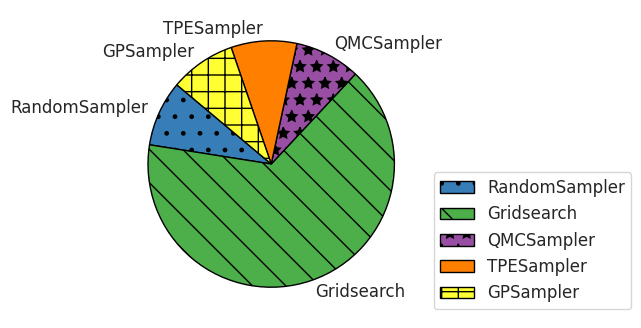
\includegraphics[width=\linewidth]{figures/predictions/sampler_distribution.png}
%     \caption{All trials training set distribution.}
%     \label{fig:sampler-distributions}
% \end{figure}



%\begin{table*}[ht!]
\centering
\caption{Default F1s for pipeline (st5, 10, UniqueMappingClustering, 0.5).}
\label{tab:global-bestf1s}
\begin{tabular}{|c|c|c|}
\toprule
Dataset & F1 & Runtime (s)\\
\midrule
D1 & 47.44 & 1.90 \\
D2 & 85.85 & 3.28 \\
D3 & 57.35 & 1.49 \\
D4 & 97.56 & 4.45 \\
D5 & 57.74 & 5.05 \\
D6 & 30.39 & 1.81 \\
D7 & 35.68 & 2.21 \\
D8 & 35.82 & 4.46 \\
D9 & 92.04 & 13.11 \\
D10 & 53.63 & 27.96 \\
\bottomrule
\end{tabular}
\end{table*}


%\subsubsection{AutoML learning procedure}

%Using auto-sklearn, we conducted experiments by withholding one dataset as the test set while training the AutoML models on all remaining datasets. The results of this approach are summarized in Table \ref{tab:autosklearn-results}, where we present the best experiments for each dataset. The column labeled \textit{Test set} indicates the dataset used as the test set, while all others served as training sets. The \textit{Trials} column lists the set of trials used for each experiment. \textit{Predicted F1} refers to the actual F1-score of the predicted configuration, measured using pyJedAI. \textit{GB-F1} represents the highest F1-score obtained by any method for each dataset, and \textit{Performance} measures how close the ETEER prediction was to the best F1-score. 
%\comments{psiliazomai, mallon swsta, ti einai to performance. mipws na dwseis ton tupo pou xreisimopoieis? vasilis: sigoura!}

%\begin{table*}[ht!]
{\footnotesize
\begin{center}  
\caption{Learning procedure 1 (AutoML) results. \textbf{WITHOUT Data Features.} GB:Gradient Boosting, RF:Random Forest, ET:Extra Trees, KNN:K-Nearest Neighbor, AD:AdaBoost, ARD:ARD Regression } 
\label{tab:autosklearn-results}
\begin{tabular}{|c|c|p{2.5cm}|c|c|c|p{2cm}|p{1.0cm}|p{1.0cm}|c|c|c|c|}
\toprule
Test set & Trials training set & Regressor ensembled & F1 & GB-F1 & F1-Ratio & Optimization \& Training time (h) & Prediction time (s) & ETEER Runtime (h) & LM & k & Clustering & Threshold \\
\midrule
D1 & all & 0.54GB + 0.36RF + 0.1GB & 57.14 & 78.43 & 0.73 & 12 & 62 & 12.02 & st5 & 1 & KMAC & 0.7790 \\
D2 & optuna & 0.92ET + 0.02ET + 0.02GB + 0.02KNN + 0.02AD & 78.63 & 85.85 & 0.92 & 12 & 61 & 12.02 & st5 & 12 & KMAC & 0.111700 \\
D3 & all & 0.62GB + 0.36RF + 0.02GB & 57.42 & 59.19 & 0.97 & 12 & 56 & 12.01 & st5 & 100 & KMAC & 0.3017 \\
D4 & all & 0.66GB + 0.32RF + 0.02GB & 98.18 & 98.60 & 1.00 & 12 & 69 & 12.02 & st5 & 21 & KMAC & 0.3019 \\
D5 & gridsearch & 0.72RF + 0.14AD + 0.12ARD + 0.02AD & 72.87 & 78.92 & 0.92 & 12 & 17 & 12.00 & st5 & 81 & KMAC & 0.70 \\
D6 & optuna & 0.86ET + 0.04ET + 0.04GB + 0.04KNN + 0.02ARD & 51.16 & 60.42 & 0.85 & 12 & 56 & 12.02 & sminilm & 1 & UMC & 0.20 \\
D7 & all & 0.58GB + 0.36RF + 0.06GB & 65.47 & 67.76 & 0.97 & 12 & 68 & 12.02 & sminilm & 1 & UMC & 0.6694 \\
D8 & optuna & 0.9ET + 0.02GB + 0.02AD + 0.02KNN + 0.02RF + 0.02RF & 47.05 & 49.53 & 0.95 & 12 & 62 & 12.02 & st5 & 1 & UMC & 0.8960 \\
D9 & optuna & 0.86ET + 0.1RF + 0.04GB & 94.39 & 94.92 & 0.99 & 12 & 25 & 12.02 & st5 & 21 & KMAC & 0.3019 \\
D10 & all & 0.6GB + 0.36RF + 0.04GB & 55.40 & 56.12 & 0.99 & 12 & 50 & 12.01 & st5 & 1 & KMAC & 0.1932 \\
\bottomrule
\end{tabular}
\end{center}  
}
\end{table*}


%Among all AutoML attempts, implementations of Gradient Boosting and Extra Trees models consistently showed the best performance. Additionally, using the \textit{all} trials set yielded the best results for 6 out of 10 datasets. However, it is also notable that the \textit{Optuna} trials sets produced the best results in 4 out of 10 datasets.

%The configurations predicted by AutoML achieved near-optimal F1-scores, particularly for datasets D2, D3, D4, D5, D7, and D9, with the minimum \textit{Performance} being 69\% "close" to the best F1-score. To further illustrate the results of this learning procedure, Figure \ref{fig:autosklearn-f1s} provides a comparative analysis of all datasets across all trial sets. There is no significant distinction between the sets of trials, as they exhibit similar performance, which is encouraging as it suggests robustness across different trial sets.
%\comments{Sto d2 kai d10 exoume kapoies diafores. eksigise giati. kapoia xaraktiristika twn datasets isws?}



%It is worth noting that the overall runtime and the runtime per model, which are auto-sklearn parameters, are dependent to the resulting performance. More time provided will result probably in an even better model selected. In our experiments, we used the predefined time limits and did not further investigate the impact of longer runtimes on AutoML's ability to find the optimal model.

%\comments{genika den sxoliazeis ka8olou kati metaksu twn datasets. kati na pros8esoume? epireazoun px ta features sto section 5.1?}

%\subsubsection{Individual regressors learning procedure}

%In a different manner, we also employed another learning procedure with quite a different methodology. We tested classic regressors provided from sklearn open-source python toolkit, while also created a naive Neural Network to test it for this task. A validation set of size 10\% from all training data trials is created, and using this we try to minimize the MSE using Optuna as a hyperparameter tool. To better understant this technique please revisit Section \ref{sec:learningProcess} and Learning Procedure 2. The exact configuarations tested can be found in Appendix and Table \ref{tab:parameter-values}. 

% \begin{table}[t]
{\footnotesize
\begin{center}  
\caption{Learning Procedure 2 results (Individual regressors).}
\label{tab:sklearn-nn-results}
\begin{tabular}{|p{0.5cm}|l|p{1.2cm}|p{1.2cm}|p{1cm}|l|}
\hline
\textbf{Test set} & \textbf{Trials} & \textbf{Regressor} & \textbf{Predicted F1} & \textbf{Best F1} & \textbf{Performance} \\
\hline
D1 & optuna & RFR & 56.77 & 78.43 & 0.72 \\
D2 & gridsearch & NN & 85.40 & 85.85 & 0.99 \\
D3 & gridsearch & XGB & 56.88 & 59.19 & 0.96 \\
D4 & all & NN & 98.51 & 98.60 & 1.00 \\
+D5 & optuna & RFR & 76.96 & 78.92 & 0.98 \\
D6 & optuna & XGB & 51.81 & 60.42 & 0.86 \\
D7 & all & RFR & 64.24 & 67.76 & 0.95 \\
D8 & all & RFR & 40.78 & 49.53 & 0.82 \\
D9 & all & RFR & 94.37 & 94.92 & 0.99 \\
D10 & all & LR & 55.80 & 56.12 & 0.99 \\
\bottomrule
\end{tabular}
\end{center}  
}
\end{table}

%\begin{table*}[ht!]
{\footnotesize
\begin{center}  
\caption{Learning procedure 2 (Linear Regression) results. \textbf{WITHOUT Data Features.}} 
\label{tab:lr-without-data-features}
\begin{tabular}{|c|c|c|c|c|c|c|c|c|c|c|c|c|}
\toprule
Test set & Trials training set & Regressor & F1 & GB-F1 & F1-Ratio & Training time (s) & Prediction time (s) & ETEER Runtime (s) & LM & k & Clustering & Threshold \\
\midrule
D1 & optuna & LR & 55.35 & 78.43 & 0.71 & 0.02 & 0.00 & 0.02 & st5 & 1 & KMAC & 0.05 \\
D2 & optuna & LR & 81.94 & 85.85 & 0.95 & 0.02 & 0.00 & 0.02 & st5 & 1 & KMAC & 0.05 \\
D3 & optuna & LR & 55.98 & 59.19 & 0.95 & 0.02 & 0.00 & 0.02 & st5 & 1 & KMAC & 0.05 \\
D4 & all & LR & 98.38 & 98.60 & 1.00 & 0.08 & 0.00 & 0.078 & st5 & 1 & KMAC & 0.05 \\
D5 & optuna & LR & 69.39 & 78.92 & 0.88 & 0.02 & 0.00 & 0.02 & st5 & 1 & KMAC & 0.05 \\
D6 & optuna & LR & 43.85 & 60.42 & 0.73 & 0.02 & 0.00 & 0.022 & st5 & 1 & KMAC & 0.05 \\
D7 & optuna & LR & 48.48 & 67.76 & 0.72 & 0.02 & 0.00 & 0.022 & st5 & 1 & KMAC & 0.05 \\
D8 & optuna & LR & 38.09 & 49.53 & 0.77 & 0.02 & 0.00 & 0.022 & st5 & 1 & KMAC & 0.05 \\
D9 & optuna & LR & 92.85 & 94.92 & 0.98 & 0.02 & 0.00 & 0.022 & st5 & 1 & KMAC & 0.05 \\
D10 & gridsearch & LR & 55.40 & 56.12 & 0.99 & 0.04 & 0.00 & 0.04 & st5 & 1 & KMAC & 0.05 \\
\bottomrule
\end{tabular}
\end{center}  
}
\end{table*} 


%Table \ref{tab:sklearn-nn-results}, shows the performance of this learning procedure. Again Random Forest is shown to be quite effective. In contrast with AutoML experiment, more trials (i.e. \textit{All} training set) yields in 6 out of 10 the best results. In a same way like the previous experiment, we provide Figure \ref{fig:sklearn-nn-f1s}, where again we notice no big differnece between sets of trials. It is now evident that no matter the trials set we will get a similar scrore, making Optunas trials set, really appealing as it has less than half the size of \textit{All} trials set.


% \subsubsection{Comparative analysis ??}

% \begin{table}[ht!]
\caption{All results (to be removed).}
\label{tab:dl-results}
\begin{tabular}{|p{0.5cm}|l|p{1.2cm}|p{1.2cm}|p{1cm}|l|}
\hline
\textbf{Test set} & \textbf{Dataset} & \textbf{Regressor} & \textbf{Predicted F1} & \textbf{Best F1} & \textbf{Perfo} \\
\hline
% \midrule
D1 & optuna & RFG & 56.77 & 78.43 & 0.72 \\
D2 & gridsearch & NN & 85.40 & 85.85 & 0.99 \\
D3 & all &  AutoGB & 57.42 & 59.19 & 0.97 \\
D4 & all & NN & 98.51 & 98.60 & 1.00 \\
D5 & optuna & RFG & 76.96 & 78.92 & 0.98 \\
D6 & optuna & XGB & 51.81 & 60.42 & 0.86 \\
D7 & all & RFG & 64.24 & 67.76 & 0.95 \\
D8 & all & RFG & 40.78 & 49.53 & 0.82 \\
D9 & optuna &  AutoET & 94.39 & 94.92 & 0.99 \\
D10 & all & LR & 55.80 & 56.12 & 0.99 \\
\bottomrule
\end{tabular}
\end{table}     


% \begin{figure}[h!]
%     \centering
%     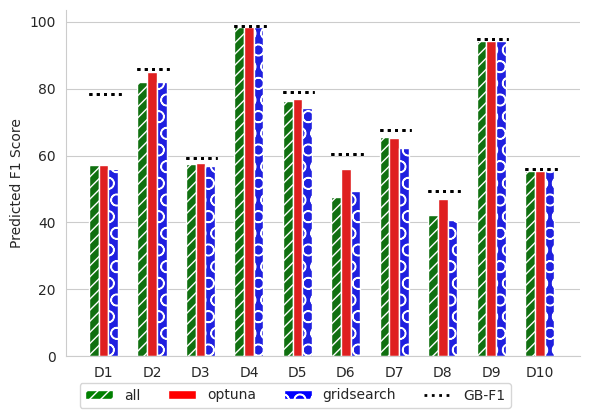
\includegraphics[width=0.99\linewidth]{figures/predictions/all_f1.png}
%     \caption{All F1-scores.}
%     \label{fig:all-f1s}
% \end{figure}

